
\newpage
\section{Einführung (2,5)}
\label{Einführung}
\subsection{Motivation}
Die Motivation dieser Arbeit ergibt sich aus der aktuellen Relevanz des Media-Mix und der zunehmenden Bedeutung von datenbasierten Marketing-Analysen. Medienverantwortliche stehen vor der Herausforderung, möglichst viele Menschen zu erreichen und den Traffic zu steigern. Gleichzeitig ist es für sie von Interesse zu verstehen, wie effektiv sie das Publikum erreichen und welchen langfristigen Einfluss einzelne Media-Kanäle auf die Nachfrage haben. Dabei dient der Nachfrageeffekt der Media-Kanäle als Grundlage für fundierte Entscheidungen.\\\\
Eine weitere Motivation besteht darin, die optimale Verteilung des Media-Budgets zu identifizieren, um sowohl eine maximale Reichweite als auch eine nachhaltige Nachfrage zu erzielen. Während in der Abteilung parallel ein Modell zur Analyse von Reichweite entwickelt wird, konzentriert sich diese Arbeit speziell auf die Untersuchung des Nachfrageeffekts. Dadurch sollen Ergebnisse bereitgestellt werden, die als Referenz für die strategische Bewertung des Media-Mix dienen können. \\
\subsection{Zielsetzung der Arbeit}
\label{ZielsetzungDerArbeit}
Das Ziel dieser Arbeit ist es, den Nachfrageeffekt verschiedener Media-Kanäle zu analysieren, um eine optimale Verteilung der Werbeausgaben zu ermöglichen. Dabei wird untersucht, wie sich die Mediaausgaben auf die Nachfrageänderung auswirken. Des Weiteren wird der \ac{ROAS} der verschiedenen Kanäle berechnet und die Verteilung der Nachfrageeffekte auf die einzelnen Media-Unterkanäle wird analysiert. Abschließend wird geprüft, ob die Ergebnisse des Marketing-Mix-Modells nachvollziehbar sind.\\\\
Die erste Fragestellung ist besonders herausfordernd, da Mediaausgaben in der Regel im Rahmen von Kampagnen getätigt werden. Dies bedeutet, dass an den meisten Tagen keine Mediaausgaben verzeichnet werden, sondern nur während der Kampagnenperioden. 
\subsection{Methodik und Ansatz}
\label{MethodikUndAnsatz}
Im Rahmen dieser Bachelorarbeit werden mehrere methodische Schritte umgesetzt. Zunächst werden die Methoden in die Arbeit integriert, darunter sowohl die lineare als auch die multiple lineare Regression, die Methode der kleinsten Quadrate und die Huber-Loss-Funktion. Ihre Funktionsweisen werden ausführlich behandelt. Anschließend erfolgt eine deskriptive Analyse der vorbereiteten Daten, um die Mediaausgaben zu untersuchen. Dabei wird auch auf die Nachvollziehbarkeit der Daten, etwa die Verteilung der Mediaausgaben, eingegangen. Weiterhin wird die Wavelet-Funktion angewendet, um die für Media relevante Nachfrage herauszufiltern. Anschließend wird eine Huber-Regression auf die gefilterten Nachfragedaten angewandt. Zur Überprüfung der Nachvollziehbarkeit und Richtigkeit der Ergebnisse erfolgt ein Austausch mit der Fachabteilung.
\subsection{Aufbau der Arbeit}
Die vorliegende Bachelorarbeit ist in fünf Kapitel unterteilt, die einen systematischen Überblick über die Forschung zu Marketing-Mix-Modell (\ac{MMM}) und die Integration der Methode der kleinsten Quadrate und Huber-Loss-Funktion geben.\\\\
Das erste Kapitel \nameref{Einführung} führt in die grundlegende Problemstellung ein und betont die Relevanz der Problemlösung für den Betrieb. In diesem Kapitel werden die Forschungsfragen aufgelistet und erklärt. Es wird beschrieben, was in dieser Arbeit erreicht wird und wie das Ziel zu erreichen ist. \\\\
Das zweite Kapitel \nameref{GeschäftlicheGrundlagen} beschreibt die Grundlagen des \ac{MMM} und definiert Media-Kanäle. Markenimage wird definiert und das Purchase-Funnel-Modell wird erklärt. Es wird auch beschrieben, welche Erfahrungen andere Unternehmen zur Kostenaufteilung in Media-Kanälen haben. Zum Schluss wird der aktuelle Stand des \ac{MMM}s bei bonprix beschrieben, und die Media-Kanäle bei bonprix werden vorgestellt. \\\\ 
Im dritten Kapitel \nameref{TheoretischeGrundlagen} wird die Methodik des Vorgehens beschrieben. Es wird erläutert, was eine deskriptive Analyse ist und wie die lineare sowie die multiple lineare Regression funktionieren. Anschließend werden die statistischen Grundlagen wie die Methode der kleinsten Quadrate, die Methode der kleinsten absoluten Abweichungen und die Huber-Loss-Funktion vorgestellt. Dazu werden auch die Einschränkungen der Regression aufgelistet, die Anpassungsgüte und die Varianzanalyse werden vorgestellt.\\\\
Das vierte Kapitel \nameref{Umsetzung} dokumentiert die Arbeitsschritte. Es fängt mit einer Vorstellung der Daten an. Die Daten werden für den Einsatz verarbeitet und die deskriptive Analyse wird eingesetzt. In der deskriptiven Analyse wird der Verlauf der Mediaausgaben und Nachfrage untersucht und die Aufteilung der Mediaausgaben wird visualisiert. Nach der deskriptiven Analyse wird die Multikollinearität zwischen den Variablen untersucht und gegebenenfalls beseitigt. Somit werden Grundlagen für die Modellierung geschaffen. Anschließend werden die Variablen in das Modell eingesetzt. Die Ergebnisse werden analysiert, und das Modell wird mit verschiedenen Kombinationen der Variablen getestet. Abschließend werden die Modellergebnisse ausgewertet und reflektiert.
\iffalse
hier nicht lesen das sind Notizen
bonprix Handelsgesellschaft mbH hat ein Marketing-Mix-Modell. Marketing-Mix-Modell quantifiziert die Effekte verschiedener Marketingtaktiken basierend auf der Nachfrage \cite{MMMdef}. Das Marketing-Mix-Modell bei bonprix umfasst die internen Faktoren, die externen Faktoren, Wettbewerber und Marketingkanäle. Media, als ein Teil von Marketingkanälen, enthält TV, Radio, Out Of Home etc. Unter Out Of Home sind alle Werbemedien im öffentlichen Raum, wie Plakate, zu verstehen. \\\\
Das Marketing-Mix-Modell differenziert nicht mehr zwischen den einzelnen Unterkanälen im Medienbereich. Wenn bonprix einen bestimmten Betrag für Medieninvestitionen ausgibt, fehlt eine Orientierung zu den Nachfrageeffekten der Unterkanäle und zur optimalen Kostenaufteilung.

bonprix zahlt einen bestimmten Betrag für das Marketing. \\ 
Es gibt 3 oberkategorien: Media, Katalog, Online-Marketing. wie viel marketing, media tv radio youtube, wenn 100mio wie viel gibt man wo aus, da am meisten investieren wo mehr nachfragen sind, 

Regressionsansatz, simple statistische regression, wie viele nachfragte durch media katalog und oma... VF aber hohe kosten, saisonalität sommer mehr und winter weniger, märz bis juli mehr nachfrage, linearer trend konjunktor, wettbewerber wenn andere mehr zahlen dann wir weniger, erklärende variablen bubbles draussen, nltrend nicht linearer trend, betas sind gewichte, beta bestimmt einfluss von einzelnen punkten, bspl oma 2,5, a ist grundnachfrage ohne alles, et ist das was man nicht erklären kann also error, saison nicht nur sommer winter in der woche auch zum beispiel WE mehr nachfrage, t ist index für Tag,
Methodik: Regression, nachfrage zerlegen in oma media...deskriptive analyse zuerst als plots, verhältnis, korrelation, parallel analysieren und schreiben, circle: daten auswahl, analyse, knowledge discovering in databases, \\ \\
Problematik: Unter Media unklar, welcher Kanal mehr Nachfrage generiert. Kosten Media = Kosten tv + Kosten ooh + Kosten radio + Youtube + Digital Media (ich weiß nicht ganz genau aber sind auch Videos online glaub ich) + OLV (Online Video) etc.
Das soll aufgesplittet werden, sodass im Modell wir jeweils einen Effekt für TV, OOH, Radio etc. haben
Ziel: media ohne Katalog? entweder ohne katalog oder bestimmte zeitrahmen aber am ende klären.  
ein mal im monat katalog schicken daher ein peak,

logit
probit
poisson
xgboosted
lasso

warum nicht früher gesplittet?

media und OMA müssen besser getrennt sein
nachfrage formel ob eher multiplikation statt plus? Moderationseffekte (=Interaktionseffekte), wenn alle Faktoren zusammenspielen/interagieren, führt es zum kauf.
mediationseffekte: ein faktor wirkt indirekt, zb Wochenende, saisonal... meistens Markenverfügbarkeit indirekt-> Nachfrage -> Markenbekanntheit, 
multiple source effect 
wie ist die nachfrage skaliert, definiert? Wie ist die Nachfrage verteilt?
histogramm: y-achse häufigkeit, x-achse ausprägungen der variablen: euro, prozent, skala wie 10/10...wann ist nachfrage gering, hoch normal...

Titel herausfinden

wavelet auch schreiben oder überspringen?


\begin{figure} [h]
    \centering
    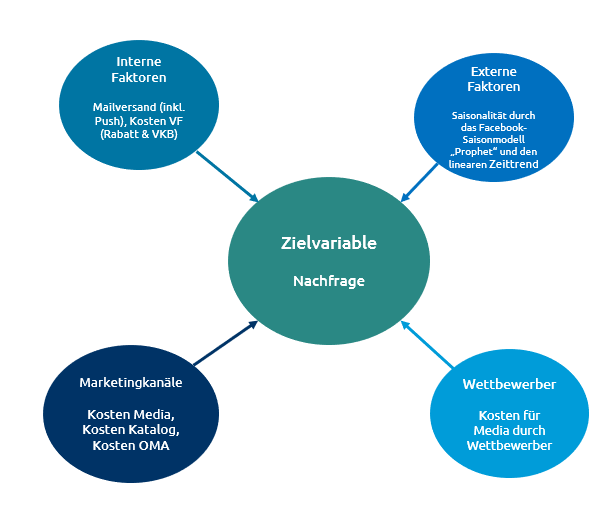
\includegraphics[width=0.75\linewidth]{mmm.png}
    \caption{\ac{MMM}-Modell bei bonprix}
    \label{fig:mmm-label}
\end{figure}


Kommentar 
\fi
